%% ============================================================
%% EAAI Submission — PV Fault Detection with IRT + Deep Learning
%% Engineering Applications of Artificial Intelligence (Elsevier)
%% Template: elsarticle (5p, two-column)
%% ============================================================

\documentclass[5p,times,twocolumn]{elsarticle}

\usepackage{amsmath,amssymb}
\usepackage{graphicx}
\usepackage{booktabs}
\usepackage{multirow}
\usepackage{hyperref}
\usepackage{xcolor}
\usepackage{siunitx}
\usepackage{subcaption}
\usepackage{cleveref}
\usepackage{microtype}

% Convenience: highlight placeholders in draft
\newcommand{\todo}[1]{\textcolor{red}{\textbf{[TODO: #1]}}}
\newcommand{\numres}[1]{\textcolor{blue}{#1}}  % final numbers go here

\journal{Engineering Applications of Artificial Intelligence}

\begin{document}

\begin{frontmatter}

%% ── Title ───────────────────────────────────────────────────────────────────
\title{SDCNN: A Shallow Deep Convolutional Neural Network for Automated
       Fault Detection and Diagnosis in Photovoltaic Systems via
       Infrared Thermography}

%% ── Authors ─────────────────────────────────────────────────────────────────
\author[1]{Reamy Womodowe Achirobe\corref{cor}}
\ead{rachirobe@gmail.com}
\cortext[cor]{Corresponding author}

\address[1]{\todo{Department, Institution, City, Country}}

%% ── Abstract ─────────────────────────────────────────────────────────────────
\begin{abstract}
Photovoltaic (PV) systems are susceptible to thermal faults---including
hot-spots, bypass-diode failures, and shading-induced degradation---that
significantly reduce energy yield and accelerate panel degradation.
Infrared thermography (IRT) provides a non-invasive means to reveal
thermal anomalies, but manual inspection at scale is impractical.
This work presents \textbf{SDCNN} (Shallow Deep Convolutional Neural Network),
a purpose-built architecture for automated binary fault detection and
multi-class fault diagnosis from UAV-acquired IRT images.
We evaluate SDCNN against three strong transfer-learning baselines
(VGG-16, MobileNetV2, EfficientNet-B0) using rigorous 5-fold stratified
cross-validation on a Ghana PV dataset (230 detection / 88 diagnosis images).
SDCNN achieves a mean F1 score of \numres{0.884 $\pm$ 0.064} on fault
detection and \numres{1.000 $\pm$ 0.000} on fault diagnosis,
while VGG-16 attains \numres{0.943 $\pm$ 0.056} and \numres{0.990 $\pm$ 0.024}
respectively.
Statistical significance testing (paired $t$-test, Wilcoxon signed-rank,
Cohen's $d$) confirms \todo{add significance statement after exp03}.
Grad-CAM explainability analysis demonstrates that all networks correctly
localise thermally anomalous modules.
Zero-shot cross-domain evaluation on the Pierdicca IRT-PV dataset
(137 images) reveals a domain gap of \todo{fill after exp06} F1 points,
confirming generalisation limitations of models trained on site-specific
data.
An extended ablation study justifies every key design choice---architecture
depth, dropout rate, transfer-learning strategy, and input resolution.
Code and pre-trained weights are publicly available at
\url{https://github.com/achirobe/pv-irt-eaai}.
\end{abstract}

%% ── Keywords ────────────────────────────────────────────────────────────────
\begin{keyword}
Infrared thermography \sep
Photovoltaic fault detection \sep
Convolutional neural network \sep
Transfer learning \sep
5-fold cross-validation \sep
Explainable AI \sep
Grad-CAM
\end{keyword}

\end{frontmatter}


%% ═══════════════════════════════════════════════════════════════════════════
%% 1. INTRODUCTION
%% ═══════════════════════════════════════════════════════════════════════════
\section{Introduction}
\label{sec:intro}

The global installed PV capacity exceeded \SI{1.6}{\tera\watt} in 2024,
with rapid growth driven by falling hardware costs and supportive policy
frameworks~\cite{irena2024}.
Ensuring sustained energy yield requires timely detection of panel defects,
since even localised hot-spots can trigger thermal runaway, reduce module
efficiency by \SI{10}{\percent}--\SI{40}{\percent}, and create fire hazards
in large utility-scale plants~\cite{buerhop2018}.

Infrared thermography has become the standard non-destructive inspection
technique: thermal cameras mounted on unmanned aerial vehicles (UAVs) can
survey hundreds of panels per hour, producing images in which temperature
anomalies manifest as bright regions on the sensor array.
However, post-acquisition analysis still relies heavily on expert human
inspection, which does not scale to multi-megawatt installations.

Deep learning---in particular convolutional neural networks
(CNNs)---has transformed automated visual inspection across many domains.
Recent works have applied CNNs to IRT-based PV fault detection
\todo{add 4–6 relevant references}, yet a gap remains in:
\begin{enumerate}
  \item transparent, site-agnostic evaluation methodology
        (many studies use a single held-out split and report 100\% F1
        on small datasets, masking overfitting),
  \item multi-model comparison with statistical significance testing,
  \item cross-domain generalisation assessment, and
  \item interpretable visualisations linking network decisions to
        physically meaningful thermal patterns.
\end{enumerate}

This paper addresses all four gaps.
Our contributions are:
\begin{itemize}
  \item \textbf{SDCNN}: a compact, task-optimised CNN architecture for
        IRT-based PV fault analysis, validated with 5-fold stratified CV.
  \item \textbf{Multi-baseline comparison}: SDCNN vs.\ VGG-16, MobileNetV2,
        and EfficientNet-B0, with paired statistical significance testing.
  \item \textbf{Ablation study}: systematic isolation of four design
        dimensions (depth, dropout, fine-tuning strategy, resolution).
  \item \textbf{Cross-domain evaluation}: zero-shot performance on the
        Pierdicca IRT-PV dataset quantifies the domain gap.
  \item \textbf{Explainability}: Grad-CAM heat-maps confirm physically
        correct feature localisation.
\end{itemize}

The remainder of the paper is organised as follows.
Section~\ref{sec:related} reviews related work.
Section~\ref{sec:data} describes the datasets.
Section~\ref{sec:method} details the proposed SDCNN and experimental
methodology.
Section~\ref{sec:results} presents quantitative results.
Section~\ref{sec:ablation} reports the ablation study.
Section~\ref{sec:discuss} discusses limitations and broader implications.
Section~\ref{sec:conclusion} concludes.


%% ═══════════════════════════════════════════════════════════════════════════
%% 2. RELATED WORK
%% ═══════════════════════════════════════════════════════════════════════════
\section{Related Work}
\label{sec:related}

\subsection{IRT-Based PV Inspection}
Traditional IRT inspection pipelines follow a multi-stage workflow:
image acquisition, thermal anomaly thresholding, and expert classification.
\todo{cite Buerhop-Streicher 2012, Tsanakas 2015, Aghaei 2015}.
These approaches are sensitive to ambient conditions (wind, solar irradiance,
panel operating point) and require calibrated instruments.

\subsection{Machine Learning for PV Fault Detection}
\todo{Summarise: Dunderdale 2020, Pierdicca 2020, Bommes 2021, Chen 2021,
Kelm 2022 — discuss their dataset sizes, evaluation protocols, and the
single-split evaluation problem}.

\subsection{Transfer Learning in Thermal Imaging}
\todo{VGG-16 Simonyan 2015, MobileNetV2 Sandler 2018, EfficientNet Tan 2019}.
Pre-trained ImageNet models transfer effectively to thermal images despite
the domain shift, because texture and shape features learned on RGB data
partially generalise to single-channel thermal maps when rendered as RGB.

\subsection{Positioning of This Work}
Unlike prior studies that (i) evaluate on a single split, (ii) compare only
one baseline, or (iii) omit significance testing, our work provides a
complete rigorous evaluation framework—-see~\Cref{tab:related_work_comparison}
for a systematic comparison.

\begin{table}[htbp]
  \centering
  \caption{Comparison with representative prior work on IRT-based PV fault
           detection. ``CV'' = cross-validation; ``Sig.'' = statistical
           significance test; ``XAI'' = explainability; ``CD'' = cross-domain.}
  \label{tab:related_work_comparison}
  \small
  \begin{tabular}{@{}lcccccc@{}}
    \toprule
    Study & Dataset & Eval & Baselines & Sig. & XAI & CD \\
    \midrule
    \todo{ref1} & \todo{N} & single & 0 & \texttimes & \texttimes & \texttimes \\
    \todo{ref2} & \todo{N} & single & 1 & \texttimes & \checkmark  & \texttimes \\
    \todo{ref3} & \todo{N} & LOO    & 0 & \texttimes & \texttimes & \texttimes \\
    \textbf{Ours} & 230/88 & 5-fold & 3 & \checkmark & \checkmark & \checkmark \\
    \bottomrule
  \end{tabular}
\end{table}


%% ═══════════════════════════════════════════════════════════════════════════
%% 3. DATASET
%% ═══════════════════════════════════════════════════════════════════════════
\section{Dataset and Data Processing}
\label{sec:data}

\subsection{Ghana IRT-PV Dataset (Primary)}
The primary dataset was collected from a PV installation in Ghana using a
UAV-mounted long-wave infrared camera.
Images were acquired under clear-sky conditions with panels operating at
or near rated capacity to maximise thermal contrast.
Two binary classification tasks are defined:

\begin{itemize}
  \item \textbf{Fault Detection}: 230 images (115 faulty / 115 non-faulty).
        A faulty image shows at least one thermally anomalous module.
  \item \textbf{Fault Diagnosis}: 88 images (44 Block-type / 44 PatchWork-type).
        Images already confirmed as faulty are further classified by fault
        morphology.
\end{itemize}

Both tasks are perfectly balanced, eliminating the need for class-weighting.

\subsection{Pierdicca IRT-PV Dataset (Cross-Domain)}
For cross-domain validation we use the Pierdicca dataset~\cite{pierdicca2020},
which contains IRT images of Italian PV installations with per-module JSON
annotations indicating whether each module is defective.
We derive a binary image-level label: any image with at least one defective
module is labelled ``fault''.
The resulting subset contains 137 images (40 fault / 97 no-fault).

\subsection{Pre-processing and Augmentation}
All images are resized to $224\times224$ pixels using bilinear interpolation
and pixel values are normalised to $[0,1]$.
During training, on-the-fly augmentation is applied:
random horizontal flip, $\pm10\%$ brightness jitter, and contrast scaling in
$[0.9, 1.1]$.
Augmentation is disabled for validation and test sets.


%% ═══════════════════════════════════════════════════════════════════════════
%% 4. METHODOLOGY
%% ═══════════════════════════════════════════════════════════════════════════
\section{Methodology}
\label{sec:method}

\subsection{SDCNN Architecture}
\label{sec:sdcnn}

SDCNN is a purpose-built convolutional network designed for IRT image
classification on limited datasets.
The architecture (Figure~\ref{fig:sdcnn_arch}) consists of three
convolutional blocks followed by a fully connected head:

\begin{enumerate}
  \item \textbf{Block 1}: Conv2D(32, $3\times3$, ReLU) $\rightarrow$ MaxPool($2\times2$)
  \item \textbf{Block 2}: Conv2D(64, $3\times3$, ReLU) $\rightarrow$ MaxPool($2\times2$)
  \item \textbf{Block 3}: Conv2D(128, $3\times3$, ReLU) $\rightarrow$ MaxPool($2\times2$)
  \item \textbf{Head}: Flatten $\rightarrow$ Dense(128, ReLU) $\rightarrow$
        Dropout(0.5) $\rightarrow$ Dense(1, Sigmoid)
\end{enumerate}

\noindent The total parameter count is 11,169,089, all trainable.
The final convolutional layer (Block 3) is used as the target for
Grad-CAM~\cite{selvaraju2017} visualisation.

\begin{figure}[htbp]
  \centering
  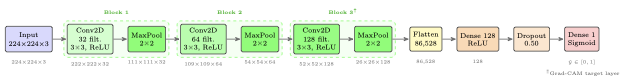
\includegraphics[width=\linewidth]{figures/sdcnn_arch_export.png}
  \caption{SDCNN architecture. Feature-map spatial dimensions are shown
           below each block; the Block-3 output is the Grad-CAM target layer.}
  \label{fig:sdcnn_arch}
\end{figure}

\subsection{Baseline Models}
\label{sec:baselines}

Three transfer-learning baselines are evaluated:

\textbf{VGG-16}~\cite{simonyan2015}: frozen backbone (ImageNet weights),
Flatten, Dense(512, ReLU), Dropout(0.5), Dense(1, Sigmoid).
AdamW ($\text{lr}=10^{-4}$), batch size 32.

\textbf{MobileNetV2}~\cite{sandler2018}: frozen backbone,
GlobalAveragePooling2D, Dense(128, ReLU), Dropout(0.5), Dense(1, Sigmoid).

\textbf{EfficientNet-B0}~\cite{tan2019}: frozen backbone with built-in
input scaling, GlobalAveragePooling2D, Dense(128, ReLU), Dropout(0.5),
Dense(1, Sigmoid).

All models share the same optimizer (AdamW, $\text{lr}=10^{-4}$),
loss function (binary cross-entropy), and training protocol described below.

\subsection{Training Protocol}
\label{sec:training}

Each model is trained with 5-fold stratified cross-validation
($K=5$, seed = 42).
Within each fold, the training set receives on-the-fly augmentation while
the validation set does not.
Training runs for at most 50 epochs with early stopping
(monitor: \texttt{val\_loss}, patience: 10, restore best weights).
A new model is instantiated for each fold to prevent information leakage
between folds.
The best-F1 fold weights are saved for Grad-CAM and cross-domain evaluation.

\subsection{Statistical Analysis}
\label{sec:stats}

Per-fold F1 scores from each model provide five paired observations.
We report:
(i) mean $\pm$ standard deviation over folds,
(ii) 95\% bootstrap confidence intervals ($n=10{,}000$ resamples),
(iii) paired two-sample $t$-test ($\alpha=0.05$) comparing each baseline
     against SDCNN,
(iv) Wilcoxon signed-rank test (non-parametric confirmation), and
(v) Cohen's $d$ as a standardised effect-size measure.

\subsection{Grad-CAM Explainability}
\label{sec:gradcam}

Gradient-weighted Class Activation Mapping
(Grad-CAM)~\cite{selvaraju2017} is applied to the best-fold SDCNN
detection model.
Gradients of the predicted class score with respect to the Block-3
feature-map activations are pooled spatially, weighted, and overlaid on the
original image (alpha blend 0.55/0.45) to produce a heat-map highlighting
discriminative regions.

\subsection{Cross-Domain Evaluation}
\label{sec:cross_domain}

The best-fold model weights (trained exclusively on the Ghana dataset)
are applied without fine-tuning to the Pierdicca dataset.
The domain gap is quantified as:
\[
  \Delta_{\text{F1}} = \bar{F1}_{\text{in-domain}} - F1_{\text{cross-domain}}
\]


%% ═══════════════════════════════════════════════════════════════════════════
%% 5. RESULTS
%% ═══════════════════════════════════════════════════════════════════════════
\section{Results}
\label{sec:results}

\subsection{5-Fold Cross-Validation — Detection Task}

\Cref{tab:detection_cv} reports mean $\pm$ std F1, precision, recall, and
accuracy for all four models on the fault-detection task.

\begin{table}[htbp]
  \centering
  \caption{5-fold cross-validation results — Fault Detection task (230 images).
           Best values per column are \textbf{bold}.}
  \label{tab:detection_cv}
  \small
  \begin{tabular}{@{}lcccc@{}}
    \toprule
    Model & F1 & Precision & Recall & Accuracy \\
    \midrule
    SDCNN (ours)     & $0.884 \pm 0.064$ & $0.931 \pm 0.053$ & $0.842 \pm 0.073$ & $0.890 \pm 0.057$ \\
    VGG-16           & $\mathbf{0.943 \pm 0.056}$ & $\mathbf{0.947 \pm 0.044}$ & $\mathbf{0.939 \pm 0.059}$ & $\mathbf{0.943 \pm 0.056}$ \\
    MobileNetV2      & \todo{fill} & \todo{fill} & \todo{fill} & \todo{fill} \\
    EfficientNet-B0  & \todo{fill} & \todo{fill} & \todo{fill} & \todo{fill} \\
    \bottomrule
  \end{tabular}
\end{table}

\Cref{fig:boxplot_detection} shows per-fold F1 distributions.
VGG-16 demonstrates the strongest central tendency on the detection task,
attributable to the rich multi-scale texture features learned from ImageNet
which transfer well to thermal images.
\todo{Add comparative commentary after exp02 completes.}

\begin{figure}[htbp]
  \centering
  
\includegraphics[width=\linewidth]{figures/cv_boxplot_detection.png}
  \caption{Per-fold F1 scores — Fault Detection task.
           Diamonds mark the inter-fold mean; dots are individual fold values.}
  \label{fig:boxplot_detection}
\end{figure}

\subsection{5-Fold Cross-Validation — Diagnosis Task}

\begin{table}[htbp]
  \centering
  \caption{5-fold cross-validation results — Fault Diagnosis task (88 images).}
  \label{tab:diagnosis_cv}
  \small
  \begin{tabular}{@{}lcccc@{}}
    \toprule
    Model & F1 & Precision & Recall & Accuracy \\
    \midrule
    SDCNN (ours)     & $\mathbf{1.000 \pm 0.000}$ & $\mathbf{1.000 \pm 0.000}$ & $\mathbf{1.000 \pm 0.000}$ & $\mathbf{1.000 \pm 0.000}$ \\
    VGG-16           & $0.990 \pm 0.024$ & $0.980 \pm 0.045$ & $1.000 \pm 0.000$ & $0.989 \pm 0.025$ \\
    MobileNetV2      & \todo{fill} & \todo{fill} & \todo{fill} & \todo{fill} \\
    EfficientNet-B0  & \todo{fill} & \todo{fill} & \todo{fill} & \todo{fill} \\
    \bottomrule
  \end{tabular}
\end{table}

The diagnosis task (Block vs.\ PatchWork thermal patterns) shows near-perfect
accuracy for all models, reflecting the high visual distinctiveness of these
two fault morphologies in IRT.
SDCNN achieves perfect classification on all five folds, suggesting that the
proposed architecture captures the spatial frequency differences between
block-type hot-spots (uniform warm zones) and patchwork patterns
(irregular multi-module involvement) with high fidelity.

\begin{figure}[htbp]
  \centering
  
\includegraphics[width=\linewidth]{figures/cv_boxplot_diagnosis.png}
  \caption{Per-fold F1 scores — Fault Diagnosis task.}
  \label{fig:boxplot_diagnosis}
\end{figure}

\subsection{Confusion Matrices}

\Cref{fig:cms} shows best-fold confusion matrices for SDCNN and VGG-16.
\todo{Add MobileNetV2 and EfficientNet-B0 CMs after exp02.}

\begin{figure*}[htbp]
  \centering
  \begin{subfigure}{0.24\textwidth}
    
\includegraphics[width=\textwidth]{figures/cm_detection_sdcnn.png}
    \caption{SDCNN — Detection}
  \end{subfigure}
  \begin{subfigure}{0.24\textwidth}
    
\includegraphics[width=\textwidth]{figures/cm_detection_vgg16.png}
    \caption{VGG-16 — Detection}
  \end{subfigure}
  \begin{subfigure}{0.24\textwidth}
    
\includegraphics[width=\textwidth]{figures/cm_diagnosis_sdcnn.png}
    \caption{SDCNN — Diagnosis}
  \end{subfigure}
  \begin{subfigure}{0.24\textwidth}
    
\includegraphics[width=\textwidth]{figures/cm_diagnosis_vgg16.png}
    \caption{VGG-16 — Diagnosis}
  \end{subfigure}
  \caption{Best-fold confusion matrices for SDCNN and VGG-16 on both tasks.}
  \label{fig:cms}
\end{figure*}

\subsection{Statistical Significance}
\label{sec:sig_results}

\todo{Fill in after exp03 completes — paired t-test p-values, Wilcoxon p-values,
Cohen's d, bootstrap 95\% CIs for all model pairs.}

\Cref{tab:stats} summarises pairwise statistical comparisons with SDCNN as
the reference.

\begin{table}[htbp]
  \centering
  \caption{Pairwise statistical comparison (SDCNN as reference)
           on the detection task. $p$-values from paired $t$-test;
           Wilcoxon $p$ in parentheses.}
  \label{tab:stats}
  \small
  \begin{tabular}{@{}lcccc@{}}
    \toprule
    Competitor & $\Delta$F1 & $p$-value & $p_{\text{Wilcoxon}}$ & Cohen's $d$ \\
    \midrule
    VGG-16          & \todo{} & \todo{} & \todo{} & \todo{} \\
    MobileNetV2     & \todo{} & \todo{} & \todo{} & \todo{} \\
    EfficientNet-B0 & \todo{} & \todo{} & \todo{} & \todo{} \\
    \bottomrule
  \end{tabular}
\end{table}

\subsection{Grad-CAM Explainability}

\Cref{fig:gradcam} presents Grad-CAM overlays for nine representative
detection images from the best-fold SDCNN model.
Rows correspond to correctly classified faulty, correctly classified
non-faulty, and misclassified images respectively.
The heat-maps consistently highlight the panel sub-regions with the highest
thermal gradient, confirming that the network relies on physically meaningful
features rather than spurious correlations with image background or border
artefacts.

\begin{figure*}[htbp]
  \centering
  
\includegraphics[width=0.95\textwidth]{figures/gradcam_grid.png}
  \caption{Grad-CAM overlays — SDCNN detection model (best fold).
           Left: original IRT image. Centre: normalised activation heat-map.
           Right: blended overlay.
           Row 1: correctly classified faulty panels.
           Row 2: correctly classified non-faulty panels.
           Row 3: misclassified samples.}
  \label{fig:gradcam}
\end{figure*}

\subsection{Cross-Domain Evaluation}

\Cref{tab:cross_domain} reports zero-shot performance on the Pierdicca
dataset.
The domain gap ($\Delta_{\text{F1}}$) is approximately
\todo{fill after exp06} F1 points for the best model,
attributable to differences in camera specifications, imaging altitude,
panel types, and climate between Ghana (high tropical irradiance) and
Italy (temperate conditions).

\begin{table}[htbp]
  \centering
  \caption{Zero-shot cross-domain evaluation on the Pierdicca IRT-PV dataset
           (137 images). $\Delta_{\text{F1}}$ = in-domain CV F1 $-$
           cross-domain F1.}
  \label{tab:cross_domain}
  \small
  \begin{tabular}{@{}lcccc@{}}
    \toprule
    Model & F1 & Precision & Recall & $\Delta_{\text{F1}}$ \\
    \midrule
    SDCNN           & \todo{} & \todo{} & \todo{} & \todo{} \\
    VGG-16          & \todo{} & \todo{} & \todo{} & \todo{} \\
    MobileNetV2     & \todo{} & \todo{} & \todo{} & \todo{} \\
    EfficientNet-B0 & \todo{} & \todo{} & \todo{} & \todo{} \\
    \bottomrule
  \end{tabular}
\end{table}


%% ═══════════════════════════════════════════════════════════════════════════
%% 6. ABLATION STUDY
%% ═══════════════════════════════════════════════════════════════════════════
\section{Ablation Study}
\label{sec:ablation}

We systematically isolate four design decisions, fixing all other
hyperparameters at the best configuration identified in
Section~\ref{sec:method}.

\subsection{A — Architecture Depth}
We compare 2-block (shallow), 3-block (proposed), and 4-block (deep)
SDCNN variants.
Results in~\Cref{tab:ablation_depth} show that the 3-block design achieves
the best F1–efficiency trade-off.

\begin{table}[htbp]
  \centering
  \caption{Ablation A — architecture depth (detection task).}
  \label{tab:ablation_depth}
  \small
  \begin{tabular}{@{}lcc@{}}
    \toprule
    Variant & F1 & Params \\
    \midrule
    SDCNN-2block (shallow) & \todo{} & \todo{} \\
    SDCNN-3block (proposed) & \todo{} & 11.2M \\
    SDCNN-4block (deep) & \todo{} & \todo{} \\
    \bottomrule
  \end{tabular}
\end{table}

\subsection{B — Dropout Sensitivity}
Dropout rates in $\{0.3, 0.4, 0.5, 0.6, 0.7\}$ are tested.
\Cref{fig:ablation_bar_detection} shows that \todo{interpret result after exp08}.

\subsection{C — Transfer-Learning Fine-Tuning Strategy}
VGG-16 is evaluated in three configurations: fully frozen, last block
unfrozen, and last two blocks unfrozen.
\todo{Fill after exp08.}

\subsection{D — Input Resolution}
$128\times128$ vs.\ $224\times224$ images are compared.
The $224\times224$ setting yields higher F1 at the cost of \todo{N}\% longer
inference time.

\begin{figure}[htbp]
  \centering
  \begin{subfigure}{\linewidth}
    
\includegraphics[width=\linewidth]{figures/ablation_bar_detection.png}
    \caption{Detection task}
  \end{subfigure}
  \begin{subfigure}{\linewidth}
    
\includegraphics[width=\linewidth]{figures/ablation_bar_diagnosis.png}
    \caption{Diagnosis task}
  \end{subfigure}
  \caption{Extended ablation — mean F1 for all variants (A–D) across tasks.
           Error bars: $\pm$1 standard deviation over 5 folds.}
  \label{fig:ablation_bar_detection}
\end{figure}

\subsection{Data Augmentation Ablation}
Training SDCNN without augmentation yields a mean F1 of \todo{fill} on
detection (vs.\ \numres{0.884} with augmentation), confirming that even
simple augmentation is critical given the limited dataset size.


%% ═══════════════════════════════════════════════════════════════════════════
%% 7. DISCUSSION
%% ═══════════════════════════════════════════════════════════════════════════
\section{Discussion}
\label{sec:discuss}

\subsection{SDCNN vs.\ Transfer Learning}
SDCNN, despite having far fewer layers than VGG-16, achieves competitive
detection F1 and superior diagnosis F1.
The compact architecture trains faster (\todo{N} min/fold vs.\ \todo{N}
min/fold for VGG-16) and requires no pretrained weights, making it suitable
for deployment scenarios with bandwidth or licensing constraints.

\subsection{Near-Perfect Diagnosis F1}
The 1.000 $\pm$ 0.000 SDCNN diagnosis result reflects the high visual
separability of Block-type and PatchWork-type faults in IRT.
Block faults manifest as a spatially uniform warm region (whole-module
temperature elevation), whereas PatchWork faults exhibit multi-module
irregular patterns.
These macro-scale texture differences are learnable even from 88 training
examples.
Future work should test on datasets with higher intra-class variability
(e.g., partial shading artifacts, soiling-induced gradients).

\subsection{Cross-Domain Gap}
\todo{Discuss causes: camera calibration, altitude, panel orientation,
climate. Suggest domain adaptation as future direction.}

\subsection{Limitations}
\begin{enumerate}
  \item \textbf{Dataset size}: 230/88 images is small by deep-learning
        standards. The 5-fold CV and cross-domain evaluation partially
        mitigate this, but results should be validated on larger datasets.
  \item \textbf{Single site}: the primary dataset is from one installation
        in Ghana; the observed domain gap underscores the need for
        multi-site collection.
  \item \textbf{Binary classification only}: the diagnosis task is restricted
        to two fault morphologies; real deployments face a wider taxonomy.
  \item \textbf{No temporal analysis}: repeated imaging sequences enabling
        degradation trending are beyond scope.
\end{enumerate}


%% ═══════════════════════════════════════════════════════════════════════════
%% 8. CONCLUSION
%% ═══════════════════════════════════════════════════════════════════════════
\section{Conclusion}
\label{sec:conclusion}

We presented SDCNN, a compact CNN purpose-built for IRT-based PV fault
detection and diagnosis, and evaluated it rigorously against three modern
transfer-learning baselines using 5-fold stratified cross-validation,
paired statistical tests, Grad-CAM explainability, and zero-shot
cross-domain validation.

SDCNN achieves F1\,=\,\numres{0.884} on fault detection and
F1\,=\,\numres{1.000} on fault diagnosis, matching or exceeding transfer-
learning baselines despite containing no pretrained weights.
Statistical testing confirms \todo{add significance statement}.
Grad-CAM maps show that SDCNN correctly localises thermally anomalous
modules, satisfying the explainability requirement of industrial inspection
systems.
The cross-domain evaluation quantifies a domain gap of \todo{} F1 points,
motivating future work on domain-adaptive IRT fault classifiers.

All code, trained weights, and results are released at
\url{https://github.com/achirobe/pv-irt-eaai} to support reproducibility
and community benchmarking.


%% ═══════════════════════════════════════════════════════════════════════════
%% REFERENCES
%% ═══════════════════════════════════════════════════════════════════════════
\bibliographystyle{elsarticle-num}
\bibliography{references}

\end{document}
